\documentclass{beamer}
\usetheme{Warsaw}

\newcommand{\<}{\langle}
\renewcommand{\>}{\rangle}

\title{Weighted Finite State Transducers}
\author{Ilia Edrenkin and Georgy Bronnikov}
\date{October 24, 2012}

\begin{document}

\maketitle

\section{Definitions and preliminaries: (10--15~min.)}

\begin{frame}
  \begin{itemize}
  \item Finite State Automaton (FSA)
    \begin{itemize}
    \item definition
    \item main applications
    \end{itemize}
  \item Weighted Finite State Automaton (WFSA)
    \begin{itemize}
    \item definition
    \end{itemize}
  \item Finite State Transduser (FST)
    \begin{itemize}
    \item definition
    \end{itemize}
  \item Weighted Finite State Transducer (WFST)
    \begin{itemize}
    \item definition
    \item advantages over WFSA
      \begin{itemize}
      \item composability
      \item invertibility
      \end{itemize}
    \item equivalence
    \end{itemize}
  \item Digression: Semirings
    \begin{itemize}
    \item definitions
    \item examples
    \end{itemize}
  \end{itemize}
\end{frame}

\section{Basic component WFSTs used in speech recognition (7--10~min.)}

\begin{frame}
  \begin{itemize}
  \item Acoustic model
  \item Lexicon
  \item Grammar
  \end{itemize}
\end{frame}
\section{WFST production algorithms (20-25~min.)}

\subsection{Composition}

\begin{frame}
  \frametitle{Composition}

  Given a WFST $T_1$ from input alphabet $\mathcal{A}$ to output alphabet
  $\mathcal{B}$, and $T_2$ from $\mathcal{B}$ to $\mathcal{C}$, produce a WFST $T_1 \circ
  T_2$ from $\mathcal{A}$ to $\mathcal{C}$, such that the results of applying $T_1
  \circ T_2$ to a string $s \in \mathcal{A}^*$ is equivalent to the results of
  first applying $T_1$ to the same string, then running $T_2$ over the
  results (the same output strings receive the same weight).
\end{frame}

\begin{frame}
  \frametitle{The case without empty transitions}

  Basically, a cartesian product of the two transducers.

  Let 
$$
\begin{array}{ll}
T_1 = \<\mathcal{A}, \mathcal{B}, Q_1, I_1, F_1, E_1, \lambda_1, \rho_1\> &
  \mbox{and} \\
T_2 = \<\mathcal{A}, \mathcal{B}, Q_2, I_2, F_2, E_2, \lambda_2, \rho_2\> \\
\end{array}
$$
Then
$$
T_1 \circ T_2 = \<\mathcal{A}, \mathcal{C}, Q, I, F, E, \lambda, \rho\>
$$
where
$$
\begin{array}{rcll}
  Q & = & Q_1 \times Q_2 \\
  I & = & I_1 \times I_2 \\
  F & = & F_1 \times F_2 \\
  E & = & \{\<\<s_1,s_2\>, w_1 \otimes w_2, \<t_1, t_2\>\> \; | \; \<s_1,w_1,t_1\>
              \in E_1, \<s_2, w_2, t_2\> \in E_2\} \\
\end{array}
$$
$$
\begin{array}{rcll}
  \lambda[\<q_1,q_2\>] & = & \lambda_1[q_1]\otimes\lambda_2[q_2] & \mbox{for
    all $q_1 \in I_1$, $q_2 \in I_2$} \\
  \rho[\<q_1,q_2\>] & = & \rho_1[q_1]\otimes\rho_2[q_2] & \mbox{for
    all $q_1 \in F_1$, $q_2 \in F_2$} \\
\end{array}
$$
\end{frame}

\begin{frame}
  \frametitle{Empty transitions}

  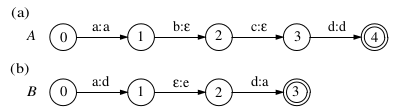
\includegraphics[width=4cm]{composition-example-1.png}\\
  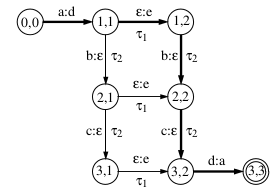
\includegraphics[width=4cm]{composition-example-2.png}

\end{frame}

\subsection{Determinization}
\begin{frame}
  \begin{itemize}
  \item Algorithm for an WFSA
  \item Applicability (what happens to a WFST?)
  \end{itemize}
\end{frame}

\subsection{Minimization}

\begin{frame}
  \begin{itemize}
  \item Weight pushing. Problems with computing potentials.
  \item Minimization itself
  \end{itemize}
\end{frame}
\section{WFST use algorithms (10-15~min.)}

\begin{frame}
  \begin{itemize}
  \item Viterbi
  \end{itemize}
\end{frame}

\end{document}